\documentclass[t]{beamer}

\usetheme{CambridgeUS}
\usecolortheme{beaver}
\setbeamertemplate{navigation symbols}{}

\usepackage[utf8]{inputenc}
\usepackage[croatian]{babel}

\usepackage{datetime}
\renewcommand{\dateseparator}{.}
\newcommand{\todayiso}{\twodigit\day \dateseparator \twodigit\month \dateseparator \the \year}
\date{\todayiso}

\usepackage{listing}
\usepackage{graphicx}
\usepackage{subcaption}
\captionsetup{compatibility=false}

\title[NKOSL]{Napredno korištenje operacijskog sustava Linux}
\author[Marin Petričević, Dominik Barbarić]{Marin Petričević, Dominik Barbarić\\{\small Nositelj: doc.dr.sc. Stjepan Groš}}
\subtitle{6. Virtualizacija}
\institute[FER]{Sveučilište u Zagrebu\\Fakultet elektrotehnike i računarstva}

\begin{document}

	{
		\setbeamertemplate{footline}{}
		\begin{frame}
			\maketitle
		\end{frame}
	}

	\begin{frame}
		\frametitle{Sadržaj}
		\tableofcontents
	\end{frame}


\section{Virtualizacija}


\begin{frame}
	\frametitle{Virtualizacija}

	\begin{itemize}
    \item Emulacija više fizickih računala na jednom
		\item Virtualizacija dijeli resurse fizičkog računala na više emuliranih računala
    \item Virtualna računala su izolirana međusobno i od fizičkog računala
	\end{itemize}

	\begin{itemize}
		\item Standardizacija produkcijske / development okoline
    \item Prenosivost okoline
    \item Lakši deployment
	\end{itemize}
\end{frame}


\begin{frame}
	\frametitle{Virtualizacija}
	\begin{columns}[T]
		\begin{column}{0.5\textwidth}
			\centering
			Bez virtualizacije\\
			\vspace{1em}
			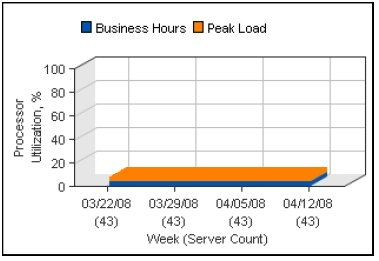
\includegraphics[width=0.9\textwidth]{no_virt_chart.jpg}
			\vspace{1em}
			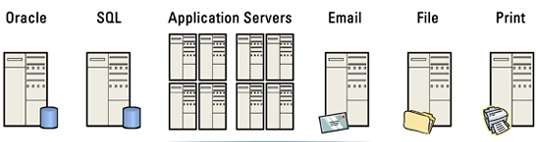
\includegraphics[width=0.8\textwidth]{no_virt_apps.jpg}
		\end{column}
		\begin{column}{0.5\textwidth}
			\centering
			Sa virtualizacijom\\
			\vspace{2em}
			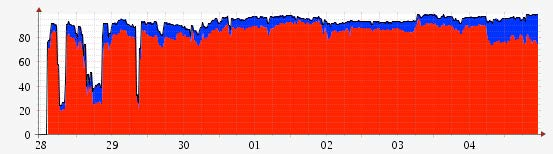
\includegraphics[width=\textwidth]{virt_chart.jpg}
			\vspace{1em}
			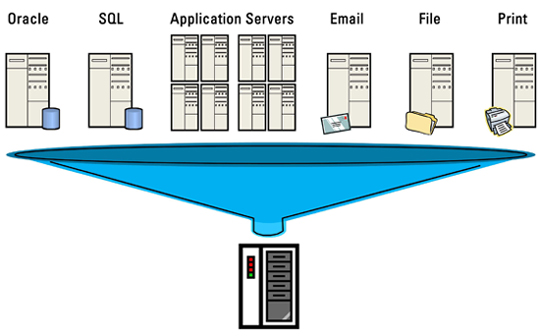
\includegraphics[width=0.9\textwidth]{virt_apps.jpg}
		\end{column}
	\end{columns}
\end{frame}




\section{Tehnike virtualizacije}

\begin{frame}
	\frametitle{Guest OS virtualizacija}
	\centering
	\begin{itemize}
		\item Virtualizaciju obavlja aplikacija unutar koje se pokreće cijeli operacijski sustav virtualnog računala
	\end{itemize}
	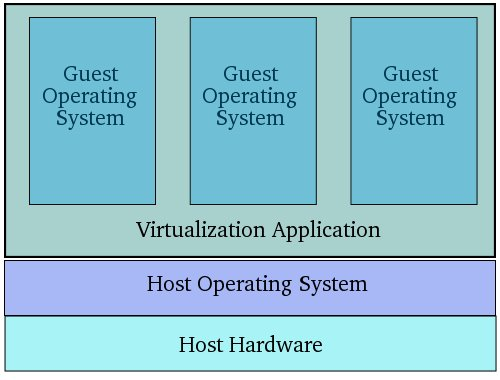
\includegraphics[width=0.65\textwidth]{guest_virt.jpg}
\end{frame}

\begin{frame}
	\frametitle{Guest OS virtualizacija}
	\centering
	\begin{itemize}
    \item VirtualBox, VMware
		\item Dobro: Lakoća korištenja, razni OSovi
    \item Loše: Performanse
	\end{itemize}
	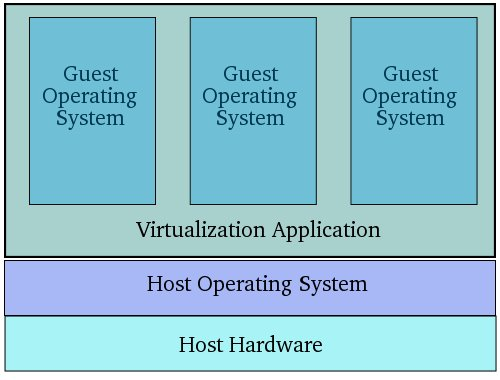
\includegraphics[width=0.60\textwidth]{guest_virt.jpg}
\end{frame}


\begin{frame}
	\frametitle{Hypervisor}
	\centering
	\begin{itemize}
		\item Operacijski sustav namijenjen virtualizaciji
	\end{itemize}
	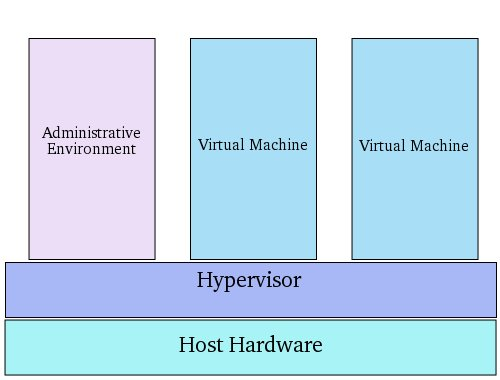
\includegraphics[width=0.65\textwidth]{hypervisor_virt.jpg}
\end{frame}

\begin{frame}
	\frametitle{Hypervisor}
	\centering
	\begin{itemize}
		\item Xen, HyperV, VMware, ...
    \item Dobro: Odlične performanse, dobra izolacija, proizvoljni OSovi
    \item Loše: Kompliciranije
	\end{itemize}
	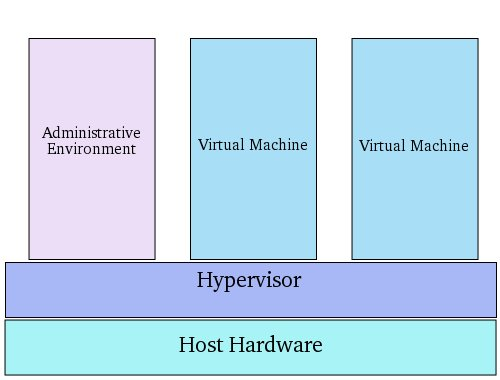
\includegraphics[width=0.65\textwidth]{hypervisor_virt.jpg}
\end{frame}


\begin{frame}
	\frametitle{Kernel virtualizacija}
	\centering
	\begin{itemize}
		\item Kernel ima podršku za virtualizaciju
    \item Vrsta hypervisora
	\end{itemize}
	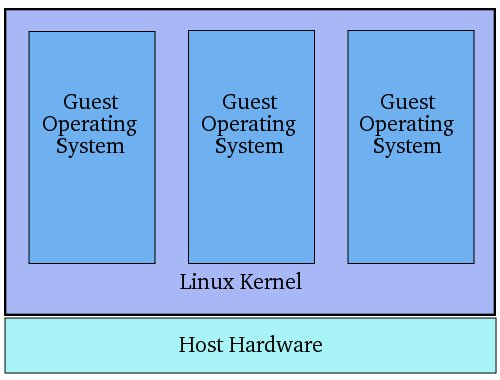
\includegraphics[width=0.65\textwidth]{kernel_virt.jpg}
\end{frame}

\begin{frame}
	\frametitle{Kernel virtualizacija}
	\centering
	\begin{itemize}
    \item KVM - Kernel-based Virtual Machine
		\item Dobro: Odlične performanse
    \item Loše: Kompliciranije, samo Linux
	\end{itemize}
	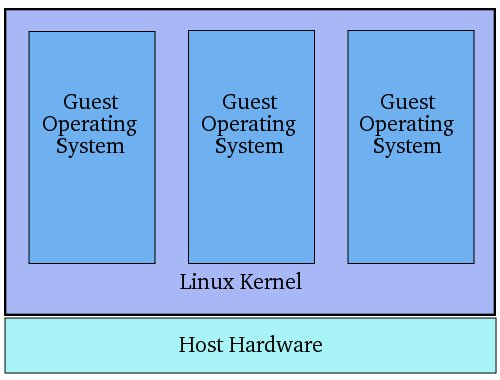
\includegraphics[width=0.60\textwidth]{kernel_virt.jpg}
\end{frame}

\begin{frame}
	\frametitle{QUEMU}
	\begin{columns}[T]
	\begin{column}{0.5\textwidth}
		\begin{itemize}
      \item Emulira različite arhitekture neovisno o arhitekturi hosta
      \item Npr. pokretanje ARM verzije linuxa na x64 procesoru
      \item Userspace virtualizator za KVM i Xen
		\end{itemize}
	\end{column}
	\begin{column}{0.5\textwidth}
		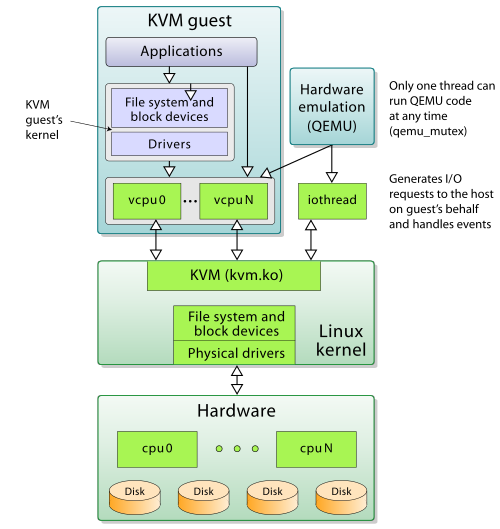
\includegraphics[width=\textwidth]{kvm.png}
	\end{column}
	\end{columns}
\end{frame}


\begin{frame}
	\frametitle{Shared kernel virtualizacija}
	\centering
	\begin{itemize}
		\item Virtualna računala dijele zajednički (Linux / UNIX) kernel
    \item Često ne koriste naziv "virtual machine" nego "container"
	\end{itemize}
	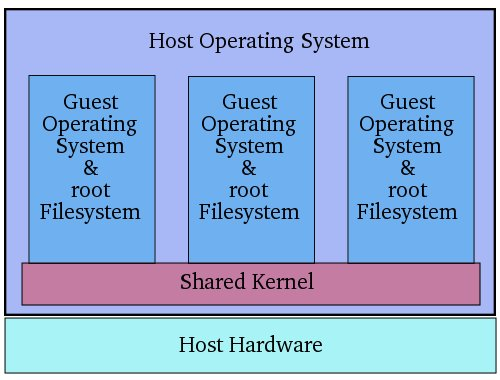
\includegraphics[width=0.60\textwidth]{shared_virt.jpg}
\end{frame}

\begin{frame}
	\frametitle{Shared kernel virtualizacija}
	\centering
	\begin{itemize}
		\item Na Linuxu: lxc, docker, runC...
    \item Drugi UNIX: FreeBSD jails, Solaris zones
    \item Dobro: lakoća korištenja, odlične performanse!
    \item Loše: Samo OSovi s kompatibilnim kernelima, nešto lošija izolacija
	\end{itemize}
	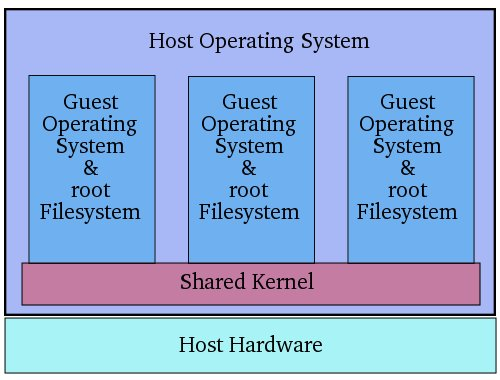
\includegraphics[width=0.45\textwidth]{shared_virt.jpg}
\end{frame}


\section{cgroups}

\begin{frame}
	\frametitle{cgroups}
	\begin{itemize}
		\item Control groups
    \item Izolacija na razini procesa - dijeljeni kernel.
	\end{itemize}
	\begin{itemize}
		\item Grupiranje procesa i razdjela resursa
		\begin{itemize}
			\item Limitiranje resursa - CPU, RAM, IO, itd.
			\item Prioriteti grupa procesa
			\item Pokretanje i zaustavljanje grupa procesa
		\end{itemize}
		\item \emph{Namespace isolation}
		\begin{itemize}
			\item \emph{Skrivanje} resursa koji nisu dodijeljeni procesu - PIDovi, mreža, file system, IPC, korisnici
      \item Skrivanjem svih resursa na host računalu se nekom procesu ili grupi procesa može dati privid da imaju računalo samo za sebe
		\end{itemize}
	\end{itemize}
\end{frame}

\begin{frame}[fragile]
	\frametitle{cgroups}
	\scriptsize
	\begin{verbatim}
# cgcreate -a user -g memory,cpu:groupname
$ ls -l /sys/fs/cgroup/memory/groupname
total 0
-rwxrwxr-x 1 user root 0 Sep 25 00:39 cgroup.event_control
-rwxrwxr-x 1 user root 0 Sep 25 00:39 cgroup.procs
-rwxrwxr-x 1 user root 0 Sep 25 00:39 cpu.rt_period_us
-rwxrwxr-x 1 user root 0 Sep 25 00:39 cpu.rt_runtime_us
-rwxrwxr-x 1 user root 0 Sep 25 00:39 cpu.shares
-rwxrwxr-x 1 user root 0 Sep 25 00:39 notify_on_release
-rwxrwxr-x 1 user root 0 Sep 25 00:39 tasks
$ cgexec   -g memory,cpu:groupname/foo bash
	\end{verbatim}

\end{frame}



\section{lxc}

\begin{frame}[fragile]
	\frametitle{LXC}

	\begin{itemize}
		\item Linux containers

		\item Shared kernel virtualizacija
		\item Implementira cgroups
	\end{itemize}

	\begin{itemize}
		\item Virtualna računala se kreiraju pomoću template skripti \texttt{/usr/share/lxc/templates}
		\item Defaultno instalacija u \texttt{/var/lib/lxc/NazivVM}
	\end{itemize}

	\scriptsize
	\begin{verbatim}
# lxc-create -n archVM -t /usr/share/lxc/templates/lxc-archlinux
# lxc-start -n archVM
# lxc-attach -n archVM
# lxc-stop -n archVM
	\end{verbatim}

\end{frame}




\section{Docker}

\begin{frame}[fragile]
	\frametitle{Docker}

	\begin{itemize}
		\item Virtualizacija na razini procesa / aplikacije
    \item Aplikaciji izgleda kao da ima OS sama za sebe
    \item Dijeli kernel sa host OSom i drugim containerima
	\end{itemize}

  \begin{itemize}
    \item Docker je više od tehnike virtualizacije, docker je ekosustav za izgradnju, deployment i upravljanje containerima
  \end{itemize}

  \begin{itemize}
    \item Docker je izolirana platforma koja sadrži sve potrebno da se pokrene neka specifična aplikacija (dependencies)
  \end{itemize}

  \scriptsize
	\begin{verbatim}
$ docker run hello-world

$ docker run -it ubuntu /bin/bash
	\end{verbatim}

\end{frame}

\begin{frame}
	\frametitle{Docker images}
	\begin{columns}[T]
	\begin{column}{0.5\textwidth}
		\begin{itemize}
      \item Srž Dockera je image sustav na copy-on-write file sustavu
      \item Hijerarhijska struktura promjena nad osnovnim datotečnim sustavom
      \item Deklarira se tekstualnom datotekom
      \item Bazini imagei dostupni na dockerhubu (hub.docker.com)
		\end{itemize}

	\end{column}
	\begin{column}{0.5\textwidth}
		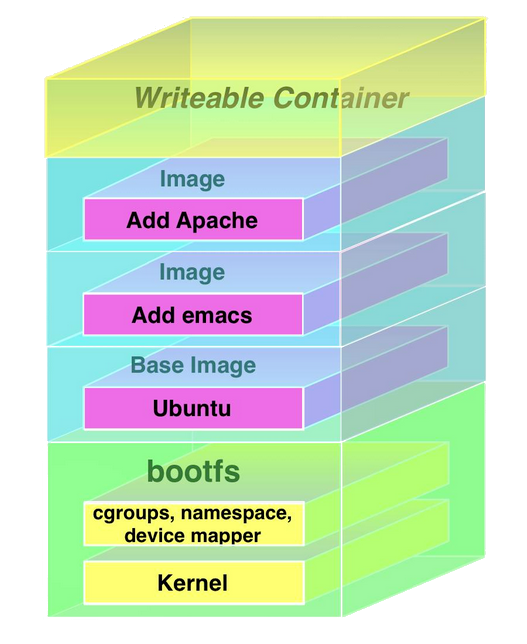
\includegraphics[width=\textwidth]{copy-on-write.png}
	\end{column}
	\end{columns}
\end{frame}


\begin{frame}[fragile]
	\frametitle{Dockerfile}
  \scriptsize
	\begin{verbatim}
FROM ruby:2.3

RUN apt-get update \
    && apt-get install -y --no-install-recommends \
        postgresql-client \
        nodejs \
    && rm -rf /var/lib/apt/lists/*

WORKDIR /usr/src/app
COPY Gemfile* ./
RUN bundle install
COPY . .
RUN bundle exec rake assets:precompile

EXPOSE 3000
CMD "./start.sh"
	\end{verbatim}
\end{frame}


\begin{frame}[fragile]
	\frametitle{Docker naredbe}

	\begin{itemize}
		\item Pregled pokrenutih containera
	\end{itemize}
  \begin{verbatim}
  $ docker ps
  \end{verbatim}

  \begin{itemize}
    \item Izgradnja Docker imagea iz foldera gdje se nalazi Dockerfile i postavljanje taga
  \end{itemize}
  \begin{verbatim}
  $ docker build -t "mojcontainer:2.0" .
  \end{verbatim}

  \begin{itemize}
    \item Pokretanje tog imagea
  \end{itemize}
  \begin{verbatim}
  $ docker run -p 3000:3000 \
               -v ./data:/app/data \
               mojcontainer:2.0 bash start.sh
  \end{verbatim}

\end{frame}


\begin{frame}[fragile]
	\frametitle{docker-compose}

  \begin{itemize}
    \item Način za pokrenuti sustav containera
    \item Tekstualna datoteka koja deklarativno opisuje ovisnosti između više containera
    \item Opisuje i sve postavke containera koje možemo upisati u command line
  \end{itemize}

  \begin{itemize}
    \item Iz foldera s \textit{docker-compose.yml} svi se containeri pokreću naredbom
  \end{itemize}

  \begin{verbatim}
  $ docker-compose up
  \end{verbatim}

\end{frame}


\begin{frame}[fragile]
	\frametitle{docker-compose.yml}

  \begin{verbatim}
services:
  db:
    image: postgres
    volumes:
      - ./db/data:/var/lib/postgresql/data
  web:
    build: .
    volumes:
      - .:/usr/src/app
    links:
      - db
    env_file: .env
    ports:
      - "3000:3000"
    restart: always
  \end{verbatim}

\end{frame}


\begin{frame}
	\frametitle{Docker at scale}

  \begin{itemize}
    \item Docker olakšava održavanje velikih sustava s redundancijom
    \item Cluster management - Desetci, stotine, tisuće servera s višestrukim instancama iste aplikacije
  \end{itemize}

  \begin{itemize}
    \item Najpopularniji alati:
    \item Docker swarm, Kubernetes, Mesos
    \item Izvan opsega NKOSLa
  \end{itemize}

\end{frame}


\begin{frame}
	\frametitle{Literatura}
	\url{http://www.virtuatopia.com/index.php/An_Overview_of_Virtualization_Techniques}
	\vfill
	\url{https://wiki.archlinux.org/index.php/Cgroups}\\
	\url{https://www.kernel.org/doc/Documentation/cgroups/cgroups.txt}
	\vfill
	\url{https://wiki.archlinux.org/index.php/Linux_Containers}
	\vfill
	\url{https://wiki.archlinux.org/index.php/QEMU}
	\vfill
	\url{http://www.linux-kvm.org/page/Main_Page}
  \vfill
  \url{https://docs.docker.com/}
\end{frame}


\end{document}
